\chapter{نظريات سرعة التفاعل}\label{ch:b3:rate-theories}

في سنة 2017 أُجيز دواء لا يختلف عن دواء أقدم إلا في
أن ذرات الهيدروجين الست في مجموعتي الميثوكسي فيه ذرات دوتيريوم. 
والكبد يفكك الدواء بقطع روابط C--H هذه بالذات، والرابطة C--D
تُقطع أبطأ بعدة مرات: فيبقى الجزيء الثقيل مدة أطول في
الدم، ويؤخذ بجرعات أصغر وأقل تواترًا. ولا شيء في قانون أرهينيوس
يفسّر لماذا يبطئ نيوترون في نواة تفاعلًا ما. يستنتج هذا
الفصل ثوابت السرعة من خواص الجزيئات: أولًا من
التصادمات، ثم من شكل \omterm{def:b3:computational-chemistry:pes}{سطح الطاقة الكامنة} ومن دوال
التجزئة في \omterm{def:b3:rate-theories:tst}{نظرية الحالة الانتقالية}، التي تتنبأ بحجم
هذه المفاعيل النظائرية؛ وينتهي بالتفاعلات في المحلول، حيث يفرض المذيب
حدًا للسرعة.

\begin{recall}
عرّف مجلد السنة الأولى ثابت السرعة، وقانون أرهينيوس $k =
A\eu^{-E_a/RT}$ بطاقة تنشيطه وعامله قبل الأسي، والخطوات
الأولية، والحالة الانتقالية، ومخطط الطاقة على امتداد إحداثي التفاعل
ومسلّمة هاموند. وعرّف مجلد السنة الثانية الشدة الأيونية ومعاملات
النشاطية، مع قانون ديباي--هوكل الحدي $\log\gamma_i = -Az_i^2\sqrt I$ ($A \approx
0.51$ في الماء عند \qty{25}{\celsius})، وضبط مستقيمات المربعات الصغرى.
وقدّم \cref{ch:b3:computational-chemistry} سطوح الطاقة الكامنة؛
وحسب \cref{ch:b3:partition-functions,ch:b3:statistical-thermo-applied}
ثوابت التوازن من دوال التجزئة وطاقات النقطة الصفرية. ومن
الفيزياء: توزيع ماكسويل--بولتزمان لسرعات الجزيئات، وقانون فيك
للانتشار.
\end{recall}

\begin{omfigure}
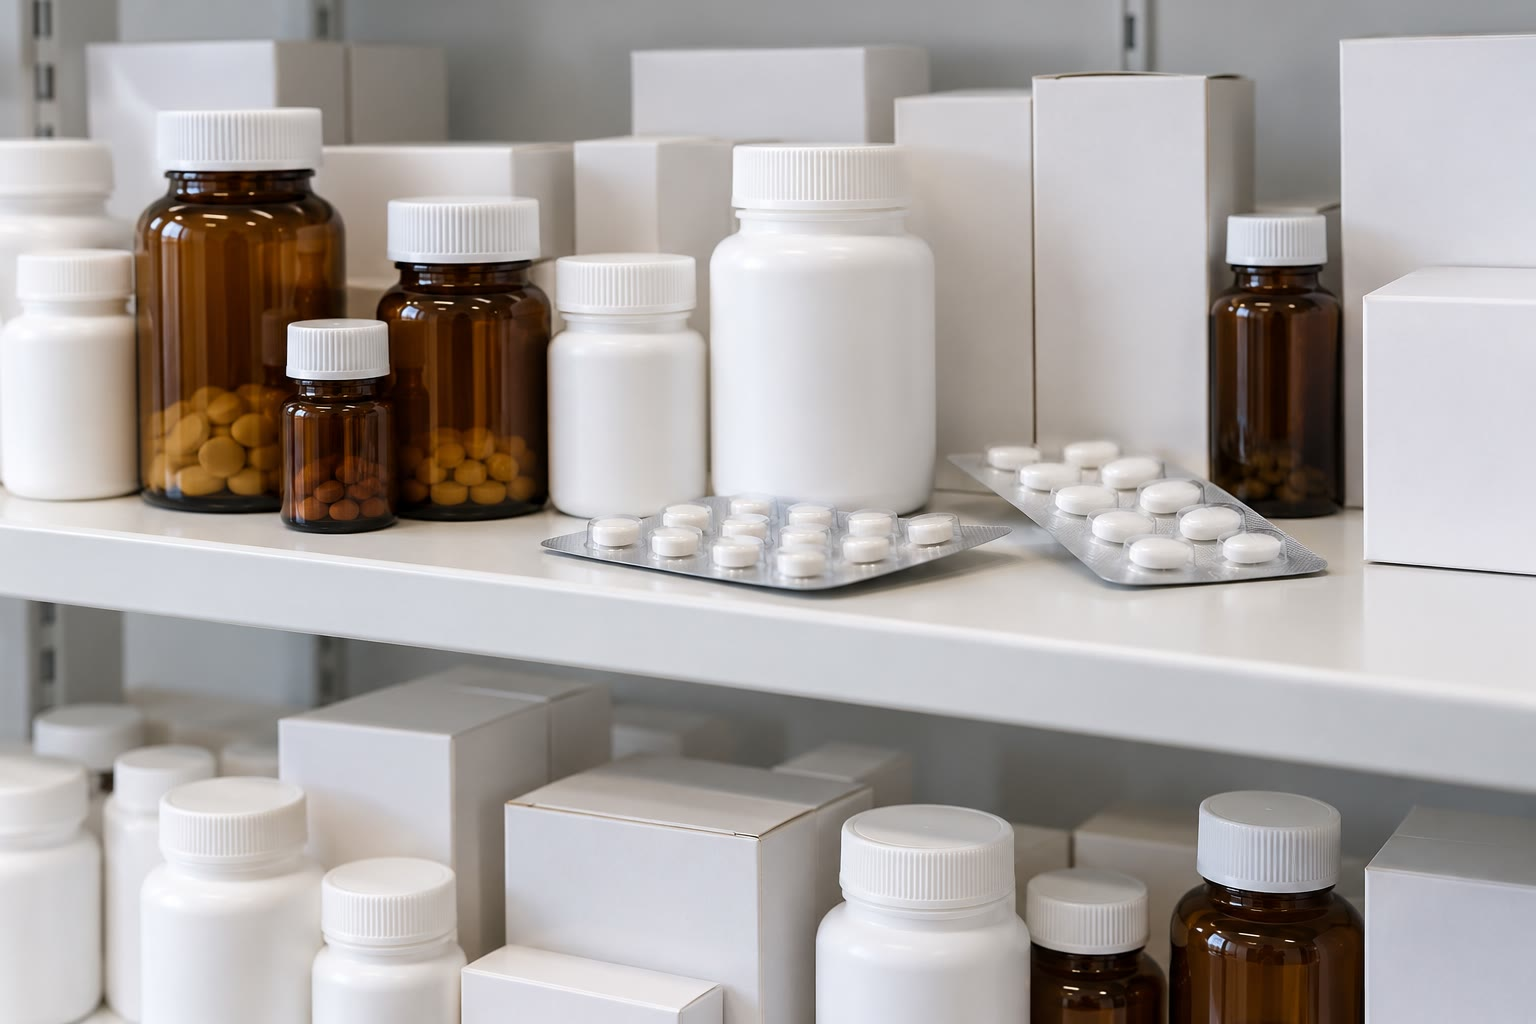
\includegraphics[width=0.6\linewidth]{images/book4/ai/b3-12-pharmacy.jpg}

{\small أدوية على رف صيدلية. استبدال الدوتيريوم بالهيدروجين في
الروابط التي يهاجمها الكبد أولًا قد يطيل مدة بقاء الدواء في الجسم.}
\end{omfigure}

\section{نظرية التصادمات}

لا يمكن لجزيئين في غاز أن يتفاعلا إلا إذا التقيا. لننمذجهما كرتين صلبتين
قطراهما $d_{\mathrm A}$ و$d_{\mathrm B}$: يتصادمان حين يمر مركزاهما على مسافة $d =
\frac12(d_{\mathrm A} + d_{\mathrm B})$ أحدهما من الآخر.

\begin{definition}[المقطع العرضي للتصادم، العامل الفراغي]\label{def:b3:rate-theories:collision}
\emph{المقطع العرضي للتصادم}\index{مقطع عرضي للتصادم} لجزيئين
هو مساحة القرص $\sigma = \pi d^2$، العمودي على سرعتهما النسبية،
الذي يجب أن يمر مركز أحدهما داخله كي يصيب الآخر. 
و\emph{العامل الفراغي}\index{عامل فراغي} $P$ هو نسبة العامل
قبل الأسي المقيس لتفاعل إلى العامل الذي تتنبأ به نظرية التصادمات.
\end{definition}

\begin{omfigure}
\begin{tikzpicture}[font=\small, >=Stealth]
  \shade[ball color=omDef!40] (0,0) circle (0.45);
  \node at (0,0) {A};
  \draw[black!50, dashed] (-0.0,0.85) -- (5.2,0.85) (-0.0,-0.85) -- (5.2,-0.85);
  \draw[black!60] (0,0) ellipse (0.25 and 0.85);
  \draw[<->] (-0.45,0) -- (-0.45,0.85) node[midway, left] {$d$};
  \shade[ball color=omThm!40] (3.3,0.55) circle (0.4);
  \node at (3.3,0.55) {B};
  \shade[ball color=omThm!20] (4.6,1.45) circle (0.4);
  \node at (4.6,1.45) {B};
  \draw[->, thick] (0.6,0) -- (2.2,0) node[midway, below] {$v_{\mathrm{rel}}\,\Delta t$};
  \node[anchor=west, align=left, font=\scriptsize] at (5.3,0) {\foreignlanguage{arabic}{أسطوانة}\\ \foreignlanguage{arabic}{مقطعها العرضي}\\ $\sigma = \pi d^2$};
  \node[font=\scriptsize, anchor=south] at (3.3,1.0) {\foreignlanguage{arabic}{إصابة}};
  \node[font=\scriptsize, anchor=south] at (4.6,1.9) {\foreignlanguage{arabic}{إخفاق}};
\end{tikzpicture}

{\small أسطوانة التصادم. يمسح الجزيء A، المتحرك بالسرعة النسبية $v_{\mathrm{rel}}$،
خلال زمن $\Delta t$ أسطوانةً مقطعها العرضي $\sigma = \pi d^2$، حيث $d$ مجموع
نصفي القطرين؛ وكل جزيء B يقع مركزه داخلها يُصاب.}
\end{omfigure}

\begin{theorem}[ثابت السرعة في نظرية التصادمات]\label{thm:b3:rate-theories:collision}
إذا كان كل تصادم تتجاوز طاقته الحركية على امتداد خط المركزين
عتبة $E_0$ (لكل مول) يؤدي إلى تفاعل، فإن ثابت سرعة $\mathrm{A + B} \to$
النواتج هو
\[
  k = \sigma\bar v_{\mathrm{rel}}N_A\,\eu^{-E_0/RT}, \qquad \bar v_{\mathrm{rel}} = \sqrt{\frac{8kT}{\pi\mu}},\
  \mu = \frac{m_{\mathrm A}m_{\mathrm B}}{m_{\mathrm A} + m_{\mathrm B}} .
\]
\end{theorem}

\begin{proof}[برهان جزئي]
في زمن $\Delta t$ يمسح جزيء A حجمًا $\sigma v_{\mathrm{rel}}\Delta t$ ويصيب جزيئات B
التي يحتويها وعددها $n_{\mathrm B}\sigma v_{\mathrm{rel}}\Delta t$: فسرعة التصادمات في وحدة الحجم
هي $\sigma\bar v_{\mathrm{rel}}n_{\mathrm A}n_{\mathrm B}$، حيث $\bar v_{\mathrm{rel}}$ متوسط السرعة النسبية الذي يعطيه
توزيع ماكسويل--بولتزمان (مأخوذ من الفيزياء، \omterm{def:b3:quantum-model-systems:oscillator}{بالكتلة
المختزلة}). وترجيح كل تصادم بسرعته والإبقاء على التصادمات التي تتجاوز طاقتها
على امتداد خط المركزين العتبة يُبقي النسبة
$\eu^{-E_0/RT}$ من سرعة التصادمات (ونقبل المكاملة على وسيط التصادم
دون برهان). وتحويل الكثافات العددية إلى تراكيز مولية يضرب في
$N_A$.
\end{proof}

بما أن $\bar v_{\mathrm{rel}} \propto \sqrt T$، فطاقة التنشيط $E_a = RT^2\,\dd\ln k/\dd T$ هي $E_0 + \frac12RT$،
قريبة من العتبة. والعامل قبل الأسي من رتبة
$10^{11}$~\unit{L.mol^{-1}.s^{-1}} للجزيئات الصغيرة. أما العوامل المقيسة فغالبًا
أصغر بكثير: $P \ll 1$ للجزيئات التي يجب أن تلتقي في
اتجاه معين، وليس للمقطع العرضي قيمة وحيدة للجزيئات الحقيقية،
التي ليست كرات صلبة. فنظرية التصادمات تعطي رتبة القدر 
وتعلق الثابت بدرجة الحرارة؛ لكنها لا تستطيع أن تعطي $E_0$، الذي يحتاج إلى \omterm{def:b3:computational-chemistry:pes}{سطح الطاقة
الكامنة}.

\section{سطوح الطاقة الكامنة}

التفاعل $\mathrm{H_A + H_BH_C \to H_AH_B + H_C}$ أبسط تفاعل على الإطلاق. ففي
اقتراب على استقامة واحدة تتعلق الطاقة بمسافتين، $r_{\mathrm{AB}}$ و$r_{\mathrm{BC}}$، ويمكن رسمها
خريطةً.

\begin{definition}[نقطة السرج، طريق الطاقة الدنيا]\label{def:b3:rate-theories:saddle}
\emph{نقطة السرج}\index{نقطة سرج} لسطح طاقة كامنة نقطة
ينعدم فيها التدرج، وتكون الطاقة عظمى في اتجاه واحد 
ودنيا في كل الاتجاهات الأخرى. و\emph{طريق الطاقة الدنيا}\index{طريق الطاقة الدنيا}
هو طريق الانحدار الأشد من نقطة السرج إلى واديي المتفاعلات
والنواتج؛ وطوله المقيس على امتداده هو إحداثي التفاعل،
ونقطة السرج هي الحالة الانتقالية.
\end{definition}

\begin{omfigure}
\begin{tikzpicture}
\begin{axis}[ompes, width=0.62\linewidth, xmin=0.4, xmax=3.0, ymin=0.4, ymax=3.0,
  xlabel={\babelsublr{$r_{\mathrm{AB}}$ / \AA}}, ylabel={\babelsublr{$r_{\mathrm{BC}}$ / \AA}},
  colorbar, colorbar style={ylabel={\babelsublr{$E$ / eV}}, ylabel style={font=\small},
  yticklabel style={font=\small}}, point meta min=-4.7, point meta max=-0.8]
\addplot3[contour prepared={labels=false}, thick] table {figdata/out/bachelor-3-pes-collinear-contours.dat};
\addplot3[ompath] table[x=x, y=y, z expr=0] {figdata/out/bachelor-3-pes-collinear-mep.dat};
\node[omsaddle] at (axis cs:0.918,0.918,0) {};
\node[font=\small, anchor=south west] at (axis cs:0.95,0.95,0) {\foreignlanguage{arabic}{نقطة السرج}};
\node[font=\small, anchor=west, fill=white, fill opacity=0.85, text opacity=1, inner sep=1.5pt] at (axis cs:2.05,1.0,0) {$\mathrm{H_A + H_BH_C}$};
\node[font=\small, anchor=west, fill=white, fill opacity=0.85, text opacity=1, inner sep=1.5pt] at (axis cs:0.95,2.55,0) {$\mathrm{H_AH_B + H_C}$};
\node[font=\small, anchor=north east] at (axis cs:2.95,2.95,0) {$\ce{H + H + H}$};
\end{axis}
\end{tikzpicture}

{\small سطح طاقة كامنة نموذجي للتفاعل $\ce{H + H2}$ على استقامة واحدة (من نوع LEPS مبني
من منحنى مورس للجزيء \ce{H2}، مع وسيط ساتو قيمته 0.17 اختير ثابتًا
نموذجيًا). خطوط التساوي من \qty{-4.65}{eV} إلى \qty{-0.8}{eV}، والطاقة معدومة لثلاث ذرات منفصلة؛
ويقع الواديان عند \qty{-4.75}{eV}، عمق بئر \ce{H2}. والمتقطع: \omterm{def:b3:rate-theories:saddle}{طريق الطاقة
الدنيا}، الذي يعبر \omterm{def:b3:rate-theories:saddle}{نقطة السرج} المتناظرة عند $r_{\mathrm{AB}} = r_{\mathrm{BC}} = \qty{0.92}{\angstrom}$،
على ارتفاع \qty{0.27}{eV} فوق الواديين في هذا النموذج.}
\end{omfigure}

يصعد الطريق من وادي المتفاعلات، حيث يبقى $r_{\mathrm{BC}}$ قرب طول رابطة
\ce{H2} بينما يقترب A، ثم يعبر \omterm{def:b3:rate-theories:saddle}{نقطة السرج}، وينزل إلى وادي
النواتج. وعند \omterm{def:b3:rate-theories:saddle}{نقطة السرج} تكون الرابطتان كلتاهما ممطوطتين إلى \qty{0.92}{\angstrom}: فالرابطة
القديمة نصف مكسورة والجديدة نصف مكوَّنة، وكلفة هذه
التسوية الطاقية هي الحاجز. وفي التفاعل المتناظر تقع \omterm{def:b3:rate-theories:saddle}{نقطة السرج} على
القطر؛ وفي التفاعل الناشر للحرارة تنتقل نحو وادي المتفاعلات (حاجز
مبكر، وحالة انتقالية شبيهة بالمتفاعلات، كما تقول مسلّمة
هاموند)، وفي التفاعل الماص للحرارة نحو وادي النواتج (حاجز متأخر).
ويحدد الموضعُ أيُّ طاقة تساعد: فالطاقة الانسحابية، الموجهة على امتداد
وادي الدخول، تحمل الجزيئات فوق الحاجز المبكر؛ أما الحاجز
المتأخر، الواقع بعد منعطف، فيُعبر بسهولة أكبر بطاقة اهتزازية في
الرابطة التي تنكسر. وهذه قواعد بولاني، التي أكدتها تجارب
الحزم الجزيئية.

\section{نظرية الحالة الانتقالية}

\begin{definition}[المعقد المنشَّط]\label{def:b3:rate-theories:activated-complex}
\emph{المعقد المنشَّط}\index{معقد منشَّط} لخطوة أولية هو
مجموعة ترتيبات النظام المتفاعل في شريحة رقيقة حول \omterm{def:b3:rate-theories:saddle}{نقطة
السرج}، عمودية على \omterm{def:b3:rate-theories:saddle}{طريق الطاقة الدنيا}؛ ويُعامل بوصفه
نوعًا كيميائيًا $\ce{AB^{\ddagger}}$، له دالة تجزئته الخاصة.
\end{definition}

\begin{definition}[نظرية الحالة الانتقالية، معامل النفاذ]\label{def:b3:rate-theories:tst}
تفترض \emph{نظرية الحالة الانتقالية}\index{نظرية الحالة الانتقالية} أن
المعقدات المنشطة في توازن مع المتفاعلات، وأن كل معقد
يعبر منطقة السرج نحو النواتج يمضي إلى تكوينها، وأن
الحركة على امتداد إحداثي التفاعل انسحاب حر. 
و\emph{معامل النفاذ}\index{معامل النفاذ} $\kappa \le 1$ يصحح من أجل
المعقدات التي تعود فتعبر نحو المتفاعلات.
\end{definition}

\begin{theorem}[معادلة أيرنغ]\label{thm:b3:rate-theories:eyring}
من أجل خطوة أولية $\mathrm{A + B} \to \mathrm{AB}^{\ddagger} \to$ النواتج،
\[
  k = \kappa\frac{k_BT}{h}\overline{K}{}^{\ddagger}, \qquad
  \overline{K}{}^{\ddagger} = \frac{\bar q^{\ddagger}/N_A}{(q_{\mathrm A}/N_A)(q_{\mathrm B}/N_A)}\,\eu^{-\Delta E_0^{\ddagger}/RT},
\]
حيث $\bar q^{\ddagger}$ دالة تجزئة \omterm{def:b3:rate-theories:activated-complex}{المعقد المنشَّط} بعد حذف حركة
إحداثي التفاعل، و$q$ دوال تجزئة مولية لوحدة
الحجم، و$\Delta E_0^{\ddagger}$ ارتفاع مستوى النقطة الصفرية للمعقد فوق
مستوى المتفاعلات. وبالصيغة الترموديناميكية، مع $c^\circ = \qty{1}{mol/L}$ 
والجزيئية $m$،
\[
  k = \kappa\frac{k_BT}{h}(c^\circ)^{1-m}\,\eu^{\Delta^{\ddagger}S^\circ/R}\,\eu^{-\Delta^{\ddagger}H^\circ/RT}.
\]
هذا القول هو \emph{معادلة أيرنغ}\index{معادلة أيرنغ}؛ و$k_B$ ثابت
بولتزمان، مكتوبًا هكذا لتجنب الخلط مع $k$.
\end{theorem}

\begin{proof}
شبه التوازن: $[\ce{AB^{\ddagger}}] = K^{\ddagger}[\mathrm A][\mathrm B]$، حيث $K^{\ddagger}$ من دوال التجزئة
(\cref{thm:b3:statistical-thermo-applied:k-from-q}، مكتوبةً بالتراكيز).
ومن اهتزازات المعقد، أحدها هو الحركة على امتداد إحداثي
التفاعل: اهتزاز رخو جدًا تردده $\nu \ll k_BT/h$، دالة تجزئته
$k_BT/h\nu$ (نهاية درجات الحرارة المرتفعة في
\cref{prop:b3:partition-functions:q-vib})؛ ومنه $q^{\ddagger} = \bar q^{\ddagger}k_BT/h\nu$. 
وتعبر المعقدات نحو النواتج بتردد هذه الحركة $\nu$، فتكون
السرعة $\nu[\ce{AB^{\ddagger}}] = \nu\frac{k_BT}{h\nu}\overline{K}{}^{\ddagger}[\mathrm A][\mathrm B]$: فيتلاشى $\nu$ المجهول. وكتابة
$\overline{K}{}^{\ddagger} = (c^\circ)^{1-m}\eu^{-\Delta^{\ddagger}G^\circ/RT}$ و$\Delta^{\ddagger}G^\circ = \Delta^{\ddagger}H^\circ - T\Delta^{\ddagger}S^\circ$ تعطي
الصيغة الثانية، مع إدخال $\kappa$ من أجل العبور العكسي.
\end{proof}

العامل $k_BT/h$ يساوي \qty{6.2e12}{s^{-1}} عند \qty{298}{K}: وهو سرعة خطوة أحادية الجزيئية
دون حاجز ودون فقد للإنتروبيا. وكل ما يخص التفاعل يكمن
في مقادير التنشيط.

\begin{definition}[طاقة جيبس للتنشيط، أنتالبي التنشيط، إنتروبيا التنشيط]\label{def:b3:rate-theories:activation}
\emph{طاقة جيبس للتنشيط}\index{طاقة جيبس للتنشيط}
$\Delta^{\ddagger}G^\circ$ و\emph{أنتالبي التنشيط}\index{أنتالبي التنشيط} $\Delta^{\ddagger}H^\circ$ 
و\emph{إنتروبيا التنشيط}\index{إنتروبيا التنشيط} $\Delta^{\ddagger}S^\circ$ لخطوة أولية
هي طاقة جيبس والأنتالبي والإنتروبيا القياسية لتكوين
\omterm{def:b3:rate-theories:activated-complex}{المعقد المنشَّط} (دون حركة إحداثي التفاعل) من المتفاعلات،
المعرَّفة \omterm{thm:b3:rate-theories:eyring}{بمعادلة أيرنغ}.
\end{definition}

\begin{proposition}[طاقة التنشيط وأنتالبي التنشيط]\label{prop:b3:rate-theories:ea-dh}
من أجل تفاعل في محلول، $E_a = \Delta^{\ddagger}H^\circ + RT$؛ ومن أجل تفاعل غازي ثنائي الجزيئية،
$E_a = \Delta^{\ddagger}H^\circ + 2RT$.
\end{proposition}

\begin{proof}
$E_a = RT^2\,\dd\ln k/\dd T$، و$\ln k = \ln T + \Delta^{\ddagger}S^\circ/R - \Delta^{\ddagger}H^\circ/RT + $ ثابت: $E_a =
RT + \Delta^{\ddagger}H^\circ$ حين لا تتغير وسائط التنشيط مع $T$. وفي المحلول
هذه هي النتيجة. أما في الطور الغازي فعلاقة فانت هوف للثابت $K^{\ddagger}$ المكتوب
بالتراكيز تتضمن الطاقة الداخلية، $\Delta^{\ddagger}U^\circ = \Delta^{\ddagger}H^\circ - \Delta n^{\ddagger}RT$
مع $\Delta n^{\ddagger} = 1 - m$: ومن أجل $m = 2$، $E_a = \Delta^{\ddagger}H^\circ + 2RT$.
\end{proof}

تقرأ \omterm{def:b3:rate-theories:activation}{إنتروبيا التنشيط} بنية الحالة الانتقالية. فجزيئان
يتحدان في معقد واحد يفقدان حرية انسحابية ودورانية:
فتكون $\Delta^{\ddagger}S^\circ$ سالبة بشدة، من $-50$ إلى $-150$ \unit{J.K^{-1}.mol^{-1}}، في
الخطوات التشاركية والحالات الانتقالية الحلقية. أما الجزيء الذي يرخي رابطة
وهو في طريقه إلى التفكك فيكسب حرية: $\Delta^{\ddagger}S^\circ > 0$.

\begin{proposition}[الأخطاء المعيارية لمستقيم مضبوط]\label{prop:b3:rate-theories:slope-uncertainty}
من أجل مستقيم مربعات صغرى $y = a + bx$ يمر بعدد $n$ من النقاط تحمل قيم $y$ فيها
أخطاء مستقلة بالتباين نفسه، المقدَّر بالعلاقة $s^2 = \sum_i(y_i - a - bx_i)^2/(n - 2)$،
يكون للميل والمقطع الخطآن المعياريان
\[
  s_b = \frac{s}{\sqrt{\sum_i(x_i - \bar x)^2}}, \qquad
  s_a = s\sqrt{\frac1n + \frac{\bar x^2}{\sum_i(x_i - \bar x)^2}} .
\]
\end{proposition}

\begin{proof}
$b = \sum_i(x_i - \bar x)y_i/S_{xx}$، حيث $S_{xx} = \sum_i(x_i - \bar x)^2$، تركيب خطي من
قيم $y_i$ مستقلة تباينها $\sigma^2$: فتباينه $\sigma^2\sum_i(x_i - \bar x)^2/S_{xx}^2 = \sigma^2/S_{xx}$.
وبالمثل $a = \bar y - b\bar x$، و$\bar y$ و$b$ غير مترابطين (تغايرهما
$\sigma^2\sum_i(x_i - \bar x)/(nS_{xx}) = 0$)، ومنه $\operatorname{var}a = \sigma^2/n + \bar x^2\sigma^2/S_{xx}$. واستبدال $\sigma^2$
بتقديره $s^2$ (والقاسم $n - 2$ يأخذ في الحسبان الوسيطين المضبوطين،
ونقبل ذلك دون برهان) يعطي النتيجة.
\end{proof}

\begin{method}[منحنى أيرنغ مع الارتيابات]\label{met:b3:rate-theories:eyring-plot}
\begin{enumerate}
  \item قِس $k$ عند خمس درجات حرارة أو أكثر موزعة على 30 إلى \qty{40}{K}.
  \item ارسم $y = \ln(k/T)$ بدلالة $x = 1/T$ واضبط مستقيم المربعات الصغرى $y = a + bx$.
  \item $\Delta^{\ddagger}H^\circ = -Rb$ و$\Delta^{\ddagger}S^\circ = R[a - \ln(k_B/h)]$ ($\ln(k_B/h) = 23.760$ مع $k$ بوحدة
        \unit{s^{-1}}).
  \item خطآهما المعياريان $Rs_b$ و$Rs_a$؛ ومجال الثقة 95\,\%
        يضربهما في معامل ستيودنت $t$ بعدد $n - 2$ من درجات الحرية (3.18 من أجل
        خمس نقاط).
  \item يقع المقطع بعيدًا خارج المجال المقيس، عند $1/T = 0$: فتكون $\Delta^{\ddagger}S^\circ$
        دائمًا أقل دقة بكثير من $\Delta^{\ddagger}H^\circ$، والخطآن
        مترابطان.
\end{enumerate}
\end{method}

\begin{omfigure}
\begin{tikzpicture}
\begin{axis}[width=0.74\linewidth, height=6.2cm, xmin=3.12, xmax=3.62, ymin=-12.8, ymax=-6.4,
  axis lines=left, xlabel={$1000\,\mathrm K/T$}, ylabel={$\ln\bigl(k/(\mathrm s^{-1}\,\mathrm K^{-1})\bigr)$},
  tick label style={font=\small}, label style={font=\small},
  legend style={font=\scriptsize, draw=none, fill=white, fill opacity=0.85, text opacity=1,
  at={(0.98,0.98)}, anchor=north east}, legend cell align=left]
\addplot[omDef, thick] table[x=invT, y=fit] {figdata/out/bachelor-3-eyring-band-H.dat};
\addplot[omThm, thick] table[x=invT, y=fit] {figdata/out/bachelor-3-eyring-band-D.dat};
\addplot[omDef, thin, dashed, forget plot] table[x=invT, y=lo] {figdata/out/bachelor-3-eyring-band-H.dat};
\addplot[omDef, thin, dashed, forget plot] table[x=invT, y=hi] {figdata/out/bachelor-3-eyring-band-H.dat};
\addplot[omThm, thin, dashed, forget plot] table[x=invT, y=lo] {figdata/out/bachelor-3-eyring-band-D.dat};
\addplot[omThm, thin, dashed, forget plot] table[x=invT, y=hi] {figdata/out/bachelor-3-eyring-band-D.dat};
\addplot[only marks, mark=*, mark size=1.8pt, omDef, forget plot] table[x=invT, y=lnkT_H] {figdata/out/bachelor-3-eyring-points.dat};
\addplot[only marks, mark=square*, mark size=1.7pt, omThm, forget plot] table[x=invT, y=lnkT_D] {figdata/out/bachelor-3-eyring-points.dat};
\legend{{\foreignlanguage{arabic}{الدواء ذو \ce{OCH3}}}, {\foreignlanguage{arabic}{الدواء ذو \ce{OCD3}}}}
\end{axis}
\end{tikzpicture}

{\small منحنيا أيرنغ لثوابت السرعة في مسألة نهاية الأسبوع (معطيات
المسألة) للدواء ولنظيره المدوتَر، مع مستقيمي المربعات الصغرى
ونطاقي الثقة 95\,\% لهما (متقطعان، لا يكادان يكونان أعرض من المستقيمين: فتشتت
النقاط نحو 1\,\%). والمستقيمان متوازيان في حدود
ارتيابهما: \omterm{def:b3:rate-theories:activation}{إنتروبيا التنشيط} نفسها، وأنتالبيا تنشيط
تختلفان بنحو \qty{5}{kJ/mol}.}
\end{omfigure}

\section{المفاعيل النظائرية الحركية}

\begin{definition}[المفاعيل النظائرية الحركية]\label{def:b3:rate-theories:kie}
\emph{المفعول النظائري الحركي}\index{مفعول نظائري حركي} لخطوة هو
النسبة $k_{\mathrm{light}}/k_{\mathrm{heavy}}$ بين ثابتي سرعتها \omterm{def:b3:rovibrational-spectroscopy:rotational-constant}{لنظيرين جزيئيين}، وغالبًا
$k_{\mathrm H}/k_{\mathrm D}$. وهو \emph{مفعول نظائري حركي أولي}\index{مفعول نظائري حركي أولي}
حين تتكون الرابطة مع الذرة المستبدلة أو تنكسر في
الخطوة، و\emph{مفعول نظائري حركي ثانوي}\index{مفعول نظائري حركي ثانوي}
حين لا يحدث ذلك.
\end{definition}

\begin{proposition}[المفعول النظائري الحركي الأولي الأعظمي]\label{prop:b3:rate-theories:primary-kie}
إذا صار اهتزاز التمدد لرابطة X--H إحداثيَّ التفاعل،
بحيث تضيع طاقة نقطته الصفرية في الحالة الانتقالية بينما تبقى كل المساهمات
الأخرى نفسها من أجل H وD، فإن
\[
  \frac{k_{\mathrm H}}{k_{\mathrm D}} = \exp\Bigl[\frac{hc(\tilde\nu_{\mathrm{XH}} - \tilde\nu_{\mathrm{XD}})}{2k_BT}\Bigr],
  \qquad \frac{\tilde\nu_{\mathrm{XH}}}{\tilde\nu_{\mathrm{XD}}} = \sqrt{\frac{\mu_{\mathrm{XD}}}{\mu_{\mathrm{XH}}}} .
\]
\end{proposition}

\begin{proof}
\omterm{def:b3:computational-chemistry:pes}{سطح الطاقة الكامنة} هو نفسه \omterm{def:b3:rovibrational-spectroscopy:rotational-constant}{للنظيرين الجزيئيين} كليهما (فالإلكترونات
لا ترى النيوترون). ففي المتفاعل يحمل تمدد \babelsublr{X--H
$\frac12hc\tilde\nu_{\mathrm{XH}}$} من \omterm{def:b3:quantum-model-systems:oscillator}{طاقة النقطة الصفرية}؛ وفي الحالة الانتقالية صار هذا النمط
إحداثي التفاعل ولا يحمل شيئًا. فالحاجز المقيس بين مستويي النقطة
الصفرية أدنى إذن بمقدار $\frac12hc\tilde\nu_{\mathrm{XH}}$ من أجل H وبمقدار $\frac12hc\tilde\nu_{\mathrm{XD}}$ من أجل D: $\Delta E_0^{\ddagger}(\mathrm D) -
\Delta E_0^{\ddagger}(\mathrm H) = \frac12hc(\tilde\nu_{\mathrm{XH}} - \tilde\nu_{\mathrm{XD}})$، وتعطي \omterm{thm:b3:rate-theories:eyring}{معادلة أيرنغ} النسبة حين
تتلاشى العوامل الأخرى. والعدد الموجي للتمدد متناسب مع
$1/\sqrt\mu$ (\cref{ch:b3:rovibrational-spectroscopy}).
\end{proof}

\begin{omfigure}
\begin{tikzpicture}[font=\small, >=Stealth, x=1cm, y=1cm]
  \draw[->] (-1.4,0) -- (-1.4,4.7) node[anchor=south] {$E$};
  \draw[->] (-1.4,0) -- (10.6,0) node[anchor=north east] {\foreignlanguage{arabic}{إحداثي التفاعل}};
  \draw[very thick, black!70] plot[smooth, tension=0.6] coordinates {(1.6,3.4) (2.1,1.6) (2.7,0.8)
    (3.3,0.6) (3.9,0.8) (4.7,2.0) (5.5,3.6) (6.2,4.0) (6.9,3.6) (7.7,2.2) (8.5,1.2) (9.2,1.0)
    (9.9,1.2) (10.4,1.7)};
  \draw[black!50, dashed] (2.8,0.6) -- (3.8,0.6);
  \draw[omDef, thick] (2.42,1.35) -- (4.2,1.35);
  \draw[omThm, thick] (2.5,1.05) -- (4.05,1.05);
  \node[omDef, font=\scriptsize, anchor=south] at (3.3,1.37) {C--H};
  \node[omThm, font=\scriptsize, anchor=north] at (3.3,1.03) {C--D};
  \draw[black, thick] (5.7,4.0) -- (6.7,4.0);
  \draw[black!40, densely dotted] (0.0,4.0) -- (5.7,4.0);
  \draw[black!40, densely dotted] (0.7,1.35) -- (2.42,1.35) (0.0,1.05) -- (2.5,1.05);
  \draw[<->, omThm] (0.0,1.05) -- (0.0,4.0) node[pos=0.5, left, font=\scriptsize] {$E_0(\mathrm D)$};
  \draw[<->, omDef] (0.7,1.35) -- (0.7,4.0) node[pos=0.5, right, font=\scriptsize] {$E_0(\mathrm H)$};
  \node[anchor=south, align=center, font=\scriptsize] at (6.2,4.05) {\foreignlanguage{arabic}{الحالة الانتقالية: صار التمدد}\\ \foreignlanguage{arabic}{إحداثيَّ التفاعل}};
\end{tikzpicture}

{\small منشأ \omterm{def:b3:rate-theories:kie}{المفعول النظائري الحركي} الأولي. في المتفاعل، يحمل تمدد C--H
طاقة نقطة صفرية أكبر مما يحمله تمدد C--D (مستويات فوق
قاع البئر، متقطع)؛ وفي الحالة الانتقالية صار هذا الاهتزاز
إحداثي التفاعل، فيبلغ النظيران الجزيئيان القمة نفسها. 
والحاجز أكبر من أجل D بمقدار الفرق بين طاقتي النقطة الصفرية.}
\end{omfigure}

\begin{omfigure}
\begin{tikzpicture}
\begin{axis}[width=0.7\linewidth, height=5.6cm, xmin=200, xmax=800, ymin=1, ymax=50,
  ymode=log, axis lines=left, xlabel={\babelsublr{$T$ / K}}, ylabel={\foreignlanguage{arabic}{$k_{\mathrm H}/k_{\mathrm D}$ الأعظمي}},
  tick label style={font=\small}, label style={font=\small}, log ticks with fixed point,
  ytick={1,2,5,10,20,50}, legend style={font=\scriptsize, draw=none, at={(0.98,0.98)},
  anchor=north east}, legend cell align=left]
\addplot[omThm, thick] table[x=T, y=OH] {figdata/out/bachelor-3-kie.dat};
\addplot[black!60, thick] table[x=T, y=NH] {figdata/out/bachelor-3-kie.dat};
\addplot[omDef, thick] table[x=T, y=CH] {figdata/out/bachelor-3-kie.dat};
\legend{{\babelsublr{O--H (\qty{3657}{cm^{-1}})}}, {\babelsublr{N--H (\qty{3337}{cm^{-1}})}}, {\babelsublr{C--H (\qty{2917}{cm^{-1}})}}}
\end{axis}
\end{tikzpicture}

{\small \omterm{def:b3:rate-theories:kie}{المفعول النظائري الحركي} الأولي الأعظمي بدلالة درجة الحرارة لفقد
تمدد C--H أو N--H أو O--H (الانتقالات الأساسية للجزيئات \ce{CH4} و\ce{NH3} و\ce{H2O}؛ 
والأعداد الموجية للدوتيريوم من الكتل المختزلة). وعند \qty{298}{K} يبلغ 6.5 للرابطة C--H؛
ويتناقص نحو 1 كلما ارتفعت درجة الحرارة.}
\end{omfigure}

القيمة العظمى للرابطة C--H في درجة حرارة الغرفة، نحو 7، معيار مرجعي. فالمفاعيل
المرصودة من 2 إلى 7 تدل على أن الرابطة C--H تنكسر في الخطوة المحددة
للسرعة؛ والقيم الأصغر على أن الحالة الانتقالية تحتفظ بجزء من التمدد
(انتقالات هيدروجين لامتناظرة، مبكرة أو متأخرة)، أو على أن الخطوة ليست
الأبطأ. أما القيم الأكبر بكثير من 7 في درجة حرارة الغرفة فلا يمكن أن تأتي من
طاقات النقطة الصفرية: إنها تكشف \omterm{def:b3:quantum-model-systems:tunnelling}{العبور النفقي} (\cref{ch:b3:quantum-model-systems})،
الذي يقوم به الجسيم ذو الكتلة المضاعفة أقل بكثير. والمفاعيل الثانوية، الناتجة عن
تغيرات اهتزازات الانحناء لروابط C--H المجاورة للمركز المتفاعل،
صغيرة، عادة من 0.8 إلى 1.2 لكل دوتيريوم؛ وهي تميّز، مثلًا،
كربونًا يصير ثلاثي الاتجاه (من \babelsublr{sp$^3$} إلى \babelsublr{sp$^2$}، $k_{\mathrm H}/k_{\mathrm D} > 1$) من كربون يصير
رباعي الأوجه ($< 1$).

\begin{method}[قياس مفعول نظائري حركي بالتنافس]\label{met:b3:rate-theories:kie}
\begin{enumerate}
  \item أجرِ التفاعل على خليط من \omterm{def:b3:rovibrational-spectroscopy:rotational-constant}{النظيرين الجزيئيين}، أو على جزيء
        يحمل H على موقع وD على موقع مكافئ.
  \item أوقف التفاعل عند تحويل منخفض وقِس نسبة نواتج H وD
        بمطيافية الكتلة أو بالرنين المغناطيسي النووي.
  \item نسبة النواتج، بعد تصحيحها بالنسبة الابتدائية، هي $k_{\mathrm H}/k_{\mathrm D}$؛ فالنظيران
        الجزيئيان يخضعان للظروف نفسها بالضبط، وهذا ما يجعل الطريقة
        أدق من قياسين منفصلين للسرعة.
\end{enumerate}
\end{method}

\section{التفاعلات في المحلول}

في السائل لا يطير الجزيء حرًا بين تصادمين: بل يتخبط في
قفص من الجيران، ويصطدم بها مرات كثيرة قبل أن ينتشر مبتعدًا.
فمتفاعلان يلتقيان يبقيان معًا تصادمات كثيرة، وهذا هو اللقاء.

\begin{definition}[التحكم بالانتشار والتحكم بالتنشيط، مفعول القفص]\label{def:b3:rate-theories:diffusion}
يكون التفاعل في المحلول \emph{محكومًا بالانتشار}\index{تفاعل محكوم بالانتشار}
حين يكون التفاعل عند كل لقاء سريعًا، فتكون سرعته هي السرعة
التي تنتشر بها المتفاعلات حتى تلتقي؛ ويكون
\emph{محكومًا بالتنشيط}\index{تفاعل محكوم بالتنشيط} حين لا يؤدي إلا جزء صغير
من اللقاءات إلى التفاعل. و\emph{مفعول القفص}\index{مفعول القفص}
هو حصر زوج من الجزيئات بالمذيب المحيط،
الذي يجعلهما يتصادمان مرارًا خلال لقاء واحد.
\end{definition}

\begin{proposition}[حد سمولوخوفسكي]\label{prop:b3:rate-theories:smoluchowski}
ثابت سرعة \omterm{def:b3:rate-theories:diffusion}{تفاعل محكوم بالانتشار} بين كرات تتفاعل
عند المسافة $R^*$ هو $k_d = 4\pi N_A(D_{\mathrm A} + D_{\mathrm B})R^*$. ومع علاقة ستوكس--أينشتاين
$D = k_BT/6\pi\eta a$ لكرات نصف قطرها $a$ في مذيب لزوجته $\eta$،
و$R^* = a_{\mathrm A} + a_{\mathrm B}$ مع $a_{\mathrm A} = a_{\mathrm B}$،
\[
  k_d = \frac{8RT}{3\eta} .
\]
\end{proposition}

\begin{proof}[برهان جزئي]
لنثبّت A في المبدأ؛ ينتشر B بمعامل الانتشار النسبي $D =
D_{\mathrm A} + D_{\mathrm B}$ ويفنى عند $r = R^*$. وفي الحالة المستقرة يكون التدفق الشعاعي
عبر كل كرة هو نفسه، $J = 4\pi r^2D\,\dd c/\dd r$ (قانون فيك، من
الفيزياء)؛ وبالمكاملة من $R^*$، حيث $c = 0$، إلى اللانهاية، حيث $c = c_{\mathrm B}$، نحصل على
$J = 4\pi DR^*c_{\mathrm B}$، وهي السرعة لكل جزيء A. ومع ستوكس--أينشتاين (المقبولة دون برهان)،
$(D_{\mathrm A} + D_{\mathrm B})R^* = \frac{k_BT}{6\pi\eta}(\frac{1}{a} + \frac1a)(2a) = \frac{2k_BT}{3\pi\eta}$، و$k_d = 4\pi N_A \times
\frac{2k_BT}{3\pi\eta} = 8RT/3\eta$.
\end{proof}

\begin{example}[حدود السرعة في الماء وفي الهكسان]\label{ex:b3:rate-theories:speed-limit}
% ledger: visc:H2O.25C, visc:hexane.25C
عند \qty{298.15}{K}، يعطي الماء ($\eta = \qty{0.890}{mPa.s}$) $k_d = 8 \times 8.314 \times
298.15/(3 \times \num{0.890e-3}) = \qty{7.4e6}{m^3.mol^{-1}.s^{-1}} = \qty{7.4e9}{L.mol^{-1}.s^{-1}}$؛ ويعطي الهكسان
($\eta = \qty{0.298}{mPa.s}$) \qty{2.2e10}{L.mol^{-1}.s^{-1}}. ولا يوجد تفاعل ثنائي الجزيئية بين
جزيئات متعادلة ذات حجم عادي أسرع من ذلك؛ والثوابت المقيسة القريبة من هذه
القيم (إخماد الحالات المثارة، واتحاد الجذور الحرة) \omterm{def:b3:rate-theories:diffusion}{محكومة
بالانتشار}. أما الأيونات ذات الشحنتين المتعاكستين فتتجاذب ويمكن أن تكون أسرع.
\end{example}

تضيف الأيونات في المحلول مساهمة كهربائية ساكنة إلى التنشيط: فالحالة
الانتقالية لأيونين شحنتها $z_{\mathrm A} + z_{\mathrm B}$، ومعامل نشاطيتها
يختلف عن جداء معاملي نشاطيتهما.

\begin{definition}[المفعول الملحي الحركي]\label{def:b3:rate-theories:salt}
\emph{المفعول الملحي الحركي}\index{مفعول ملحي حركي} هو تغيّر ثابت
سرعة تفاعل بين أيونات مع الشدة الأيونية للمحلول.
\end{definition}

\begin{proposition}[معادلة برونستد--بييروم]\label{prop:b3:rate-theories:bronsted-bjerrum}
من أجل خطوة بين أيونين شحنتاهما $z_{\mathrm A}$ و$z_{\mathrm B}$ في محلول مائي مخفف،
\[
  \log k = \log k_0 + 2Az_{\mathrm A}z_{\mathrm B}\sqrt I,
\]
حيث $k_0$ ثابت السرعة عند شدة أيونية معدومة.
\end{proposition}

\begin{proof}
في \omterm{def:b3:rate-theories:tst}{نظرية الحالة الانتقالية} يُكتب التوازن مع \omterm{def:b3:rate-theories:activated-complex}{المعقد المنشَّط}
بالنشاطيات: $[\ce{AB^{\ddagger}}] = K^{\ddagger}[\mathrm A][\mathrm B]\gamma_{\mathrm A}\gamma_{\mathrm B}/\gamma^{\ddagger}$، ومنه $k = k_0\gamma_{\mathrm A}\gamma_{\mathrm B}/\gamma^{\ddagger}$.
ومع القانون الحدي: $\log(\gamma_{\mathrm A}\gamma_{\mathrm B}/\gamma^{\ddagger}) = -A\sqrt I[z_{\mathrm A}^2 + z_{\mathrm B}^2 - (z_{\mathrm A} + z_{\mathrm B})^2] =
2Az_{\mathrm A}z_{\mathrm B}\sqrt I$.
\end{proof}

الأيونات ذات الإشارة الواحدة تتفاعل أسرع حين يُضاف ملح (فالجو الأيوني
يحجب تنافرها)، والأيونات ذات الإشارتين المتعاكستين أبطأ، والمتفاعل
المتعادل لا يُظهر أي مفعول ملحي أولي: فمنحنى $\log k$ بدلالة $\sqrt I$ عند
الشدة الأيونية المنخفضة يقيس جداء شحنات الأنواع المتفاعلة.

\begin{method}[ما تقوله وسائط التنشيط عن الآلية]\label{met:b3:rate-theories:mechanism-evidence}
\begin{enumerate}
  \item $\Delta^{\ddagger}S^\circ$ سالبة بشدة: خطوة تشاركية، أو حالة انتقالية منتظمة أو حلقية،
        أو حالة تنظّم المذيب (تولّد شحنات)؛
        وموجبة: خطوة تفككية.
  \item $k_{\mathrm H}/k_{\mathrm D}$ أولي من 2 إلى 7: الرابطة مع H تنكسر في
        الخطوة المحددة للسرعة؛ وفوق نحو 10 في درجة حرارة الغرفة: \omterm{def:b3:quantum-model-systems:tunnelling}{عبور نفقي}.
  \item ميل $\log k$ بدلالة $\sqrt I$: جداء الشحنتين $z_{\mathrm A}z_{\mathrm B}$ اللتين
        تلتقيان في الخطوة المحددة للسرعة.
  \item ثابت سرعة قرب $10^{10}$~\unit{L.mol^{-1}.s^{-1}} يتغير كالمقدار $T/\eta$:
        تحكم بالانتشار.
\end{enumerate}
\end{method}

\begin{inthelab}[خلية بغلاف مزدوج لدراسة أيرنغ]
يُتتبع التفاعل بامتصاصيته في خلية مقياس طيف ضوئي يُغذّى
غلافها بحمام منظَّم الحرارة؛ ويتحقق مزدوج حراري في خلية مرجعية من
درجة الحرارة بدقة \qty{0.1}{K}. وخمس إلى سبع درجات حرارة، يُقاس كل منها
ثلاث مرات، تعطي منحنى أيرنغ؛ وتُترك المحاليل حتى تتوازن حراريًا في
الحامل قبل المزج، لأن تفاعلًا يبدأ عند درجة حرارة خاطئة يحرف
النقاط الأولى.
\end{inthelab}

\begin{history}[أيرنغ وإيفانز وبولاني، 1935]
في سنة 1935 نشر هنري أيرنغ، في برينستون، وميريديث غوين إيفانز ومايكل
بولاني، في مانشستر، كلٌّ على حدة نظرية \omterm{def:b3:rate-theories:activated-complex}{المعقد
المنشَّط}. وكان أيرنغ قد حسب، مع بولاني في برلين سنة 1931، أول
سطح طاقة كامنة للتفاعل $\ce{H + H2}$، بطريقة نصف تجريبية من النوع المستعمل
لشكل هذا الفصل. وقوبلت النظرية بالريبة: فقد رفضت
مجلة أولًا مقالة أيرنغ بوصفها غير سليمة، ولم تُنشر إلا
بعد أن شهد لها فيزيائيون آخرون.
\end{history}

\section{تمارين}

\begin{exercise}[$\star$]\label{exo:b3:rate-theories:1}
% ledger: kin:NO+O3.A
من أجل $\ce{NO + O3 -> NO2 + O2}$ خذ $\sigma = \qty{0.43}{nm^2}$ (معطيات التمرين). احسب $\bar v_{\mathrm{rel}}$
عند \qty{298}{K} ($\mu = \qty{18.46}{u}$)، والعامل قبل الأسي في نظرية التصادمات، 
\omterm{def:b3:rate-theories:collision}{والعامل الفراغي} علمًا أن $A = \qty{2.07e-12}{cm^3.s^{-1}}$ المقيس لكل جزيء.
\end{exercise}

\begin{exercise}[$\star$]\label{exo:b3:rate-theories:2}
لتفاعل في محلول $E_a = \qty{75.0}{kJ/mol}$ قرب \qty{298}{K}. ما $\Delta^{\ddagger}H^\circ$؟ وما هي
لتفاعل غازي ثنائي الجزيئية له $E_a$ نفسها؟
\end{exercise}

\begin{exercise}[$\star$]\label{exo:b3:rate-theories:3}
تنبأ بإشارة $\Delta^{\ddagger}S^\circ$ في: إضافة حلقية من نوع ديلز--ألدر؛ 
والفقد الأحادي الجزيئية للجزيء \ce{N2} من مركب آزوي؛ وتفاعل $\mathrm{S_N2}$ بين جزيئين
متعادلين يولّد أيونين في مذيب قطبي.
\end{exercise}

\begin{exercise}[$\star$]\label{exo:b3:rate-theories:4}
% ledger: visc:H2O.25C, visc:hexane.25C
احسب ثابت السرعة \omterm{def:b3:rate-theories:diffusion}{المحكوم بالانتشار} في الماء وفي الهكسان عند
\qty{298.15}{K}. أي المذيبين يسمح بلقاءات أسرع، ولماذا؟
\end{exercise}

\begin{exercise}[$\star\star$]\label{exo:b3:rate-theories:5}
لتفاعل من الرتبة الأولى $k = \qty{1.00e-3}{s^{-1}}$ عند \qty{298.15}{K} و\qty{1.00e-2}{s^{-1}} عند
\qty{318.15}{K}. احسب $\Delta^{\ddagger}H^\circ$ و$\Delta^{\ddagger}S^\circ$، و$E_a$ للمقارنة.
\end{exercise}

\begin{exercise}[$\star\star$]\label{exo:b3:rate-theories:6}
% ledger: vib:H2O.sym
احسب المفعول النظائري الأولي الأعظمي لنقل بروتون O--H عند
\qty{298}{K} ($\tilde\nu_{\mathrm{OH}} = \qty{3657}{cm^{-1}}$، والكتل المختزلة مع O = 16، H = 1، D = 2).
\end{exercise}

\begin{exercise}[$\star\star$]\label{exo:b3:rate-theories:7}
% ledger: vib:CH4.nu1, vib:CD4.nu1
يُظهر نقل هيدروجين إنزيمي من الكربون $k_{\mathrm H}/k_{\mathrm D} = 40$ عند \qty{298}{K}. قارن
بالقيمة العظمى المحسوبة من طاقات النقطة الصفرية ($\tilde\nu = 2917$ و\qty{2109}{cm^{-1}}) واستنتج.
\end{exercise}

\begin{exercise}[$\star\star$]\label{exo:b3:rate-theories:8}
تنبأ بأثر رفع الشدة الأيونية من 0 إلى 0.010 في سرعة: أكسدة \ce{I-}
بالأيون \ce{S2O8^{2-}} (الخطوة المحددة للسرعة بين هذين الأيونين)؛ 
وتفاعل \ce{CH3COOC2H5} مع \ce{OH-}؛ وتفاعل $\ce{[Co(NH3)5Br]^{2+}}$ مع \ce{OH-}.
وأعطِ العامل حيث يوجد ($A = 0.51$).
\end{exercise}

\begin{exercise}[$\star\star$]\label{exo:b3:rate-theories:9}
التفاعل $\ce{F + H2 -> HF + H}$ ناشر للحرارة بشدة. أين يقع حاجزه على
\omterm{def:b3:computational-chemistry:pes}{سطح الطاقة الكامنة}؟ ومن أجل التفاعل العكسي، أي صورة من صور الطاقة، تُعطى
للمتفاعلات، تساعده أكثر؟
\end{exercise}

\begin{exercise}[$\star\star\star$]\label{exo:b3:rate-theories:10}
يعطي ضبط المربعات الصغرى للمقدار $\ln(k/T)$ بدلالة $1/T$ على خمس نقاط $b = -7446$ K
مع $s_b = \qty{31}{K}$ و$a = 16.528$ مع $s_a = 0.103$. أعطِ $\Delta^{\ddagger}H^\circ$ و$\Delta^{\ddagger}S^\circ$ مع
خطأيهما المعياريين ومجالي الثقة 95\,\% ($t = 3.18$).
\end{exercise}

\begin{exercise}[$\star\star\star$]\label{exo:b3:rate-theories:11}
انطلاقًا من \omterm{thm:b3:rate-theories:eyring}{معادلة أيرنغ}، بيّن أن $E_a = \Delta^{\ddagger}H^\circ + RT$ لخطوة
أحادية الجزيئية وأن $A = \eu\,(k_BT/h)\eu^{\Delta^{\ddagger}S^\circ/R}$. واستنتج $A$ من أجل $\Delta^{\ddagger}S^\circ = 0$ عند
\qty{298}{K}، وقارنه بالقيم $10^{13}$ إلى $10^{14}$~\unit{s^{-1}} لانشطارات الروابط البسيطة.
\end{exercise}

\begin{exercise}[$\star\star\star$]\label{exo:b3:rate-theories:12}
طبّق \omterm{def:b3:rate-theories:tst}{نظرية الحالة الانتقالية} على ذرتين عديمتي البنية A وB يكون معقدهما
المنشَّط جزيئًا ثنائي الذرة طول رابطته $d$ (لا اهتزاز يبقى بعد حذف إحداثي
التفاعل، ودوران مع $I = \mu d^2$). بيّن أنها تعطي
ثابت السرعة في نظرية التصادمات مع $\sigma = \pi d^2$.
\end{exercise}

\section{مسألة: دواء أثقل}

\begin{problem}[{مسألة نهاية الأسبوع --- دواء أثقل: طاقات النقطة الصفرية
لتمددي C--H وC--D، والمفعول النظائري الأعظمي عند درجة حرارة الجسم، 
وزمن نصف العمر لدواء مدوتَر، وتحليل أيرنغ للمركبين كليهما}]
\label{pb:b3:rate-theories:1}
% ledger: vib:CH4.nu1, vib:CD4.nu1, imass:H1, imass:H2, hist4:deut.2017
يُطرح دواء من الجسم بطريقين: 75\,\% من طرحه بنزع الميثيل عن
مجموعتي \ce{OCH3} فيه، حيث يكون قطع رابطة C--H الخطوة
المحددة للسرعة، و25\,\% بطرق لا تمس هذه الروابط؛ وزمن نصف
عمره \qty{5.0}{h} (معطيات المسألة). ويحمل نظيره مجموعتي \ce{OCD3}.
نماذج تمددي C--H وC--D: التمددان المتناظران للجزيئين \ce{CH4}
(\qty{2917}{cm^{-1}}) و\ce{CD4} (\qty{2109}{cm^{-1}}). وثوابت السرعة من الرتبة الأولى لخطوة
نزع الميثيل المقيسة بمستحضر إنزيمي كبدي (معطيات
المسألة):
\begin{center}\small
\begin{tabular}{lccccc}
\hline
\babelsublr{$T$ / K} & 278.15 & 288.15 & 298.15 & 308.15 & 318.15 \\
\babelsublr{$k_{\mathrm H}$ / \unit{s^{-1}}} & 0.00989 & 0.0263 & 0.0632 & 0.150 & 0.328 \\
\babelsublr{$k_{\mathrm D}$ / \unit{s^{-1}}} & 0.00117 & 0.00333 & 0.00874 & 0.0219 & 0.0503 \\ \hline
\end{tabular}
\end{center}

\medskip\noindent\textbf{الجزء الأول --- طاقات النقطة الصفرية.}
\begin{enumerate}
  \item احسب الكتلتين المختزلتين للرابطتين C--H وC--D (C = 12، H = 1.00783،
        D = 2.01410).
  \item تنبأ بالعدد الموجي للرابطة C--D انطلاقًا من عدد C--H وقارنه بالقيمة
        المقيسة \qty{2109}{cm^{-1}}.
  \item احسب طاقتي النقطة الصفرية للتمددين والفرق بينهما،
        بوحدة \unit{cm^{-1}} و\unit{kJ/mol} (بالأعداد الموجية المقيسة).
  \item ماذا يحدث لاهتزاز تمدد الرابطة التي تنكسر في
        الحالة الانتقالية؟
  \item استنتج الفرق بين الحاجزين من أجل H وD.
\end{enumerate}

\medskip\noindent\textbf{الجزء الثاني --- المفعول النظائري.}
\begin{enumerate}[resume]
  \item احسب القيمة العظمى للنسبة $k_{\mathrm H}/k_{\mathrm D}$ عند \qty{37}{\celsius}.
  \item احسبها عند \qty{25}{\celsius}.
  \item لماذا تسمى قيمة عظمى؟
  \item هل تساهم ذرتا الدوتيريوم الأخريان في كل مجموعة \ce{CD3} مساهمة كبيرة؟
  \item ماذا تقول قيمة مقيسة قرب 7 عند \qty{25}{\celsius} عن
        الآلية؟
\end{enumerate}

\medskip\noindent\textbf{الجزء الثالث --- أزمنة نصف العمر.}
\begin{enumerate}[resume]
  \item كيف يتعلق زمن نصف العمر بثابت سرعة الطرح الكلي؟
  \item اكتب ثابت السرعة الكلي لدواء H مجموعًا لطريقيه،
        بالنسب.
  \item بكم يتباطأ طريق نزع الميثيل في دواء D؟
  \item احسب $k_{\mathrm{total}}(\mathrm D)/k_{\mathrm{total}}(\mathrm H)$.
  \item احسب زمن نصف عمر دواء D.
  \item احسب نسبة زمني نصف العمر.
  \item ماذا تكون لو مرّ الطرح كله عبر نزع الميثيل؟
  \item ماذا يغيّر زمن نصف عمر أطول بالنسبة إلى المريض؟
\end{enumerate}

\medskip\noindent\textbf{الجزء الرابع --- تحليل أيرنغ.}
\begin{enumerate}[resume]
  \item أي تمثيل بياني للمعطيات يكون خطيًا بحسب \omterm{thm:b3:rate-theories:eyring}{معادلة أيرنغ}؟
  \item اضبطه لدواء H: $\Delta^{\ddagger}H^\circ$ و$\Delta^{\ddagger}S^\circ$ مع خطأيهما المعياريين.
  \item افعل الشيء نفسه لدواء D.
  \item احسب $\Delta\Delta^{\ddagger}H^\circ = \Delta^{\ddagger}H^\circ(\mathrm D) - \Delta^{\ddagger}H^\circ(\mathrm H)$ وخطأه المعياري.
  \item هل يساوي الفرق بين طاقتي النقطة الصفرية في السؤال 3؟
  \item ماذا تقول \omterm{def:b3:rate-theories:activation}{إنتروبيا التنشيط} في الحالتين؟
  \item اذكر النتيجة: النسبة المتنبأ بها بين زمني نصف عمر الدواءين
        عند \qty{37}{\celsius}.
\end{enumerate}
\end{problem}
